\begin{savequote}[8cm]

	"I've made peace with myself."\newline
	"Good for you. That's the hardest war of all to win."\newline
	"Didn't say I won. Just stopped fighting."\newline
	\qauthor{―-- Joe Abercrombie, \textit{Best Served Cold}}
\end{savequote}

\chapter{Discussion and Conclusions}

% \subsection{The Ancestral Recombination Graph (ARG) and admixture inference in the ancient past}


% The phylogenetic trees over a set of samples as they change along the genome through recombination, collectively referred to as the ancestral recombination graph (ARG) \cite{Griffiths1997a,Rasmussen2014}, record all information about the samples' evolutionary history.  This history itself is shaped by the population's demography, a statistical relationship that is quantified by the coalescent-with-recombination (CwR) model \cite{Griffiths1997a}.  The ARG is a complex data structure which is only weakly constrained by the observed genetic polymorphisms, making inference of demography difficult. By making approximations to the CwR, for instance by making an independent-sites assumption, efficient parametric inference of demography becomes possible \cite{Excoffier2013,McVean2005}.  Methods including {\tt PSMC} \cite{Li2011}, {\tt diCal} \cite{Steinrucken2015} and {\tt SMC++} \cite{Terhorst2015} allow non-parametric inference of demography under a closer approximation to the CwR, but one that does not include gene flow between populations. MSMC \cite{Schiffels2014} introduced the cross-coalescent rate and {\tt MSMC-IM} described how to interpret this rate in the context of a isolation-migration model to estimate a migration rate between populations\cite{Wang2019a}. However, these methods are not well suited for estimating directional migration rates. 

% Here we extend SMCSMC (Sequential Monte Carlo inference of the Sequentially Markovian Coalescent, \cite{Henderson2018}) to allow inference of directional migration.  SMCSMC is a Bayesian method that uses a particle filter to explicitly sample from the posterior distribution of ARGs over multiple diploid samples under the full CwR model.
% Since particle filters operate by simulating latent variables (here the ARG) under the statistical model of interest, it becomes possible to handle complex demographic scenarios.  We exploit this by extending the CwR model to include time-varying directional migration rates in a two-island demographic model.  We use the posterior sample of ARGs including migration events to update the parameters of the demographic model, using either expectation-maximization or a variational Bayes procedure, and iterate these steps until convergence.   We apply SMCSMC to estimate directional migration rates in whole genome sequencing data from the Simons Genome Diversity Panel (SGDP) \cite{Mallick2016} and the Human Genome Diversity Panel (HGDP) \cite{Bergstrom2019} to investigate population structure around the OoA event.

% \subsection{Migration initialisation Values} \label{ch2:initial}

% We select a more comprehensive set of initiation pardameters and particle values and use them to analyze a Yoruban and French individual from SGDP (Fig \ref{init_yri}). The effect of the initial migration rate seems relatively consistent for low values (0.5 - 2.0),while an increasingly small migration peak is seen for higher initial magnitudes 4.0 - 10.0. Again, beginning with an initial rate of zero tends to lead to highly unstable estimates of effective population size and migration rates. For the remainder of the analyses in this article, we choose to use an initial rate of 1.0. 



% \begin{figure}
% 	\centering
% 	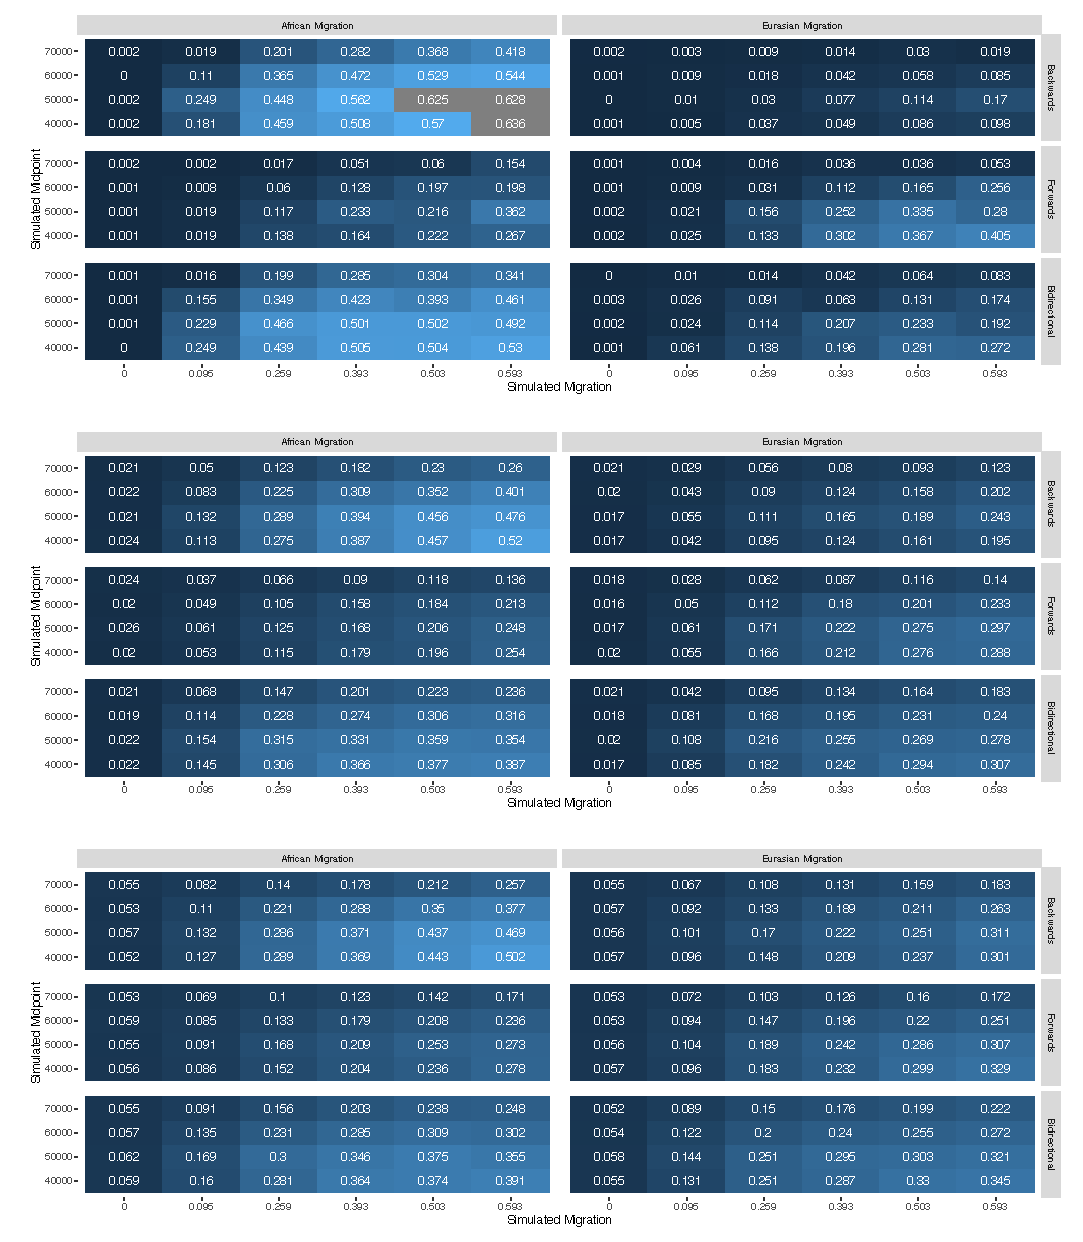
\includegraphics[width=\textwidth]{plot/all_integrated_sims.pdf}
% 	\caption[Integrated migration for three cases of simulated demographies]{ {\bf Integrated migration fraction (IMF) in the last 100ky for three cases of simulated demography shown in \ref{fig:backsim}, \ref{fig:bisim}, and \ref{fig:fwdsim}.} Simulations were performed as per Supplemental Section \ref{methods:simproc} with an additional parameter for the initial migration rate used to initialise the SMCSMC particle filter. The timing and IMF simulated are as per the aforementioned figures. From top to bottom, inference was initiated with 0, 1, and 5 4$N_0$ population replacement per generation in the specified direction (backwards, bidirectionally, and forwards).}
% 	\label{fig:intsim}
% \end{figure}

% \begin{figure}
% 	\centering
% 	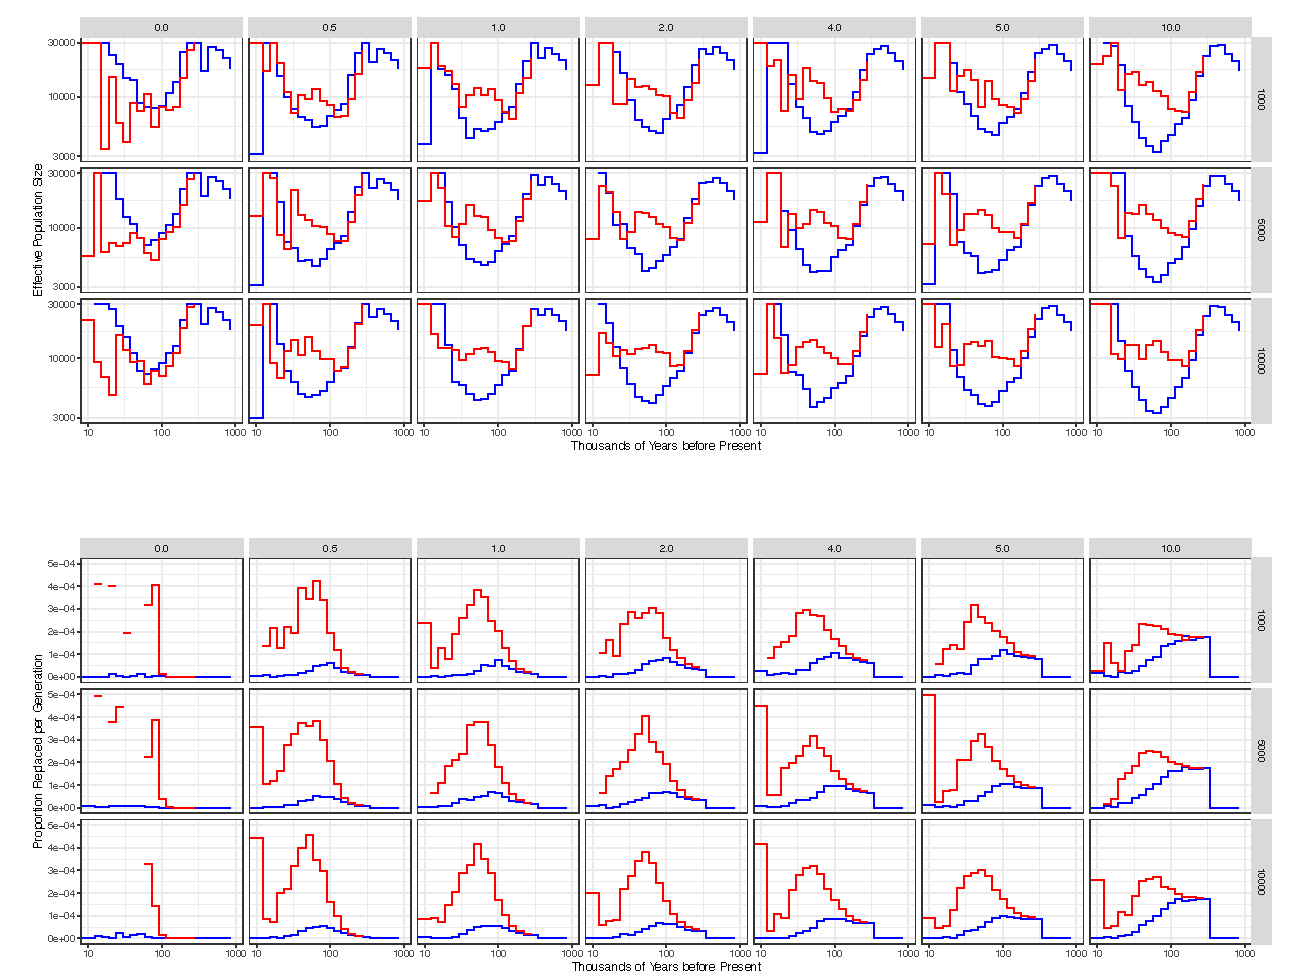
\includegraphics[width=\textwidth]{plot/yri_dif_migs.pdf}
% 	\caption[The effect of initial mirgation on demographic inference]{ {\bf The effect of initial migration parameter on demographic inference.} Effective population size and migration history of a Yoruban ({\tt S\_Yoruba-1}) and a French ({\tt S\_French-1}) individual from the Simons Genome Diversity panel were modelled with SMCSMC. The initial migration proportion, in units of 4 $N_0$ proportion of the population replaced per generation was varied along the X axis, while the number of particles is varied along the Y. 10 iterations of variational Bayes was used for parameter inference, while 5000 particles were used infer the ancestral recombination graph.}
% 	\label{fig:init_yri}
% \end{figure}

% \minitoc

